\begin{quote}
This is part 24 of Categories for Programmers. Previously:
\href{https://bartoszmilewski.com/2017/01/02/comonads/}{Comonads}. See
the
\href{https://bartoszmilewski.com/2014/10/28/category-theory-for-programmers-the-preface/}{Table
of Contents}.
\end{quote}

We've seen several formulations of a monoid: as a set, as a
single-object category, as an object in a monoidal category. How much
more juice can we squeeze out of this simple concept?

Let's try. Take this definition of a monoid as a set \texttt{m} with a
pair of functions:

\begin{verbatim}
μ :: m × m -> m η :: 1 -> m
\end{verbatim}

Here, 1 is the terminal object in \textbf{Set} --- the singleton set.
The first function defines multiplication (it takes a pair of elements
and returns their product), the second selects the unit element from
\texttt{m}. Not every choice of two functions with these signatures
results in a monoid. For that we need to impose additional conditions:
associativity and unit laws. But let's forget about that for a moment
and just consider ``potential monoids.'' A pair of functions is an
element of a cartesian product of two sets of functions. We know that
these sets may be represented as exponential objects:

\begin{verbatim}
μ ∈ m m×m η ∈ m1
\end{verbatim}

The cartesian product of these two sets is:

\begin{verbatim}
m m×m × m1
\end{verbatim}

Using some high-school algebra (which works in every cartesian closed
category), we can rewrite it as:

\begin{verbatim}
m m×m + 1
\end{verbatim}

The plus sign stands for the coproduct in \textbf{Set}. We have just
replaced a pair of functions with a single function --- an element of
the set:

\begin{verbatim}
m × m + 1 -> m
\end{verbatim}

Any element of this set of functions is a potential monoid.

The beauty of this formulation is that it leads to interesting
generalizations. For instance, how would we describe a group using this
language? A group is a monoid with one additional function that assigns
the inverse to every element. The latter is a function of the type
\texttt{m-\textgreater{}m}. As an example, integers form a group with
addition as a binary operation, zero as the unit, and negation as the
inverse. To define a group we would start with a triple of functions:

\begin{verbatim}
m × m -> m m -> m 1 -> m
\end{verbatim}

As before, we can combine all these triples into one set of functions:

\begin{verbatim}
m × m + m + 1 -> m
\end{verbatim}

We started with one binary operator (addition), one unary operator
(negation), and one nullary operator (identity --- here zero). We
combined them into one function. All functions with this signature
define potential groups.

We can go on like this. For instance, to define a ring, we would add one
more binary operator and one nullary operator, and so on. Each time we
end up with a function type whose left-hand side is a sum of powers
(possibly including the zeroth power --- the terminal object), and the
right-hand side being the set itself.

Now we can go crazy with generalizations. First of all, we can replace
sets with objects and functions with morphisms. We can define n-ary
operators as morphisms from n-ary products. It means that we need a
category that supports finite products. For nullary operators we require
the existence of the terminal object. So we need a cartesian category.
In order to combine these operators we need exponentials, so that's a
cartesian closed category. Finally, we need coproducts to complete our
algebraic shenanigans.

Alternatively, we can just forget about the way we derived our formulas
and concentrate on the final product. The sum of products on the left
hand side of our morphism defines an endofunctor. What if we pick an
arbitrary endofunctor \texttt{F} instead? In that case we don't have to
impose any constraints on our category. What we obtain is called an
F-algebra.

An F-algebra is a triple consisting of an endofunctor \texttt{F}, an
object \texttt{a}, and a morphism

\begin{verbatim}
F a -> a
\end{verbatim}

The object is often called the carrier, an underlying object or, in the
context of programming, the carrier \emph{type}. The morphism is often
called the evaluation function or the structure map. Think of the
functor \texttt{F} as forming expressions and the morphism as evaluating
them.

Here's the Haskell definition of an F-algebra:

\begin{verbatim}
type Algebra f a = f a -> a
\end{verbatim}

It identifies the algebra with its evaluation function.

In the monoid example, the functor in question is:

\begin{verbatim}
data MonF a = MEmpty | MAppend a a
\end{verbatim}

This is Haskell for \texttt{1\ +\ a\ ×\ a} (remember
\href{https://bartoszmilewski.com/2015/01/13/simple-algebraic-data-types/}{algebraic
data structures}).

A ring would be defined using the following functor:

\begin{verbatim}
data RingF a = RZero | ROne | RAdd a a | RMul a a | RNeg a
\end{verbatim}

which is Haskell for \texttt{1\ +\ 1\ +\ a\ ×\ a\ +\ a\ ×\ a\ +\ a}.

An example of a ring is the set of integers. We can choose
\texttt{Integer} as the carrier type and define the evaluation function
as:

\begin{verbatim}
evalZ :: Algebra RingF Integer evalZ RZero = 0 evalZ ROne = 1 evalZ (RAdd m n) = m + n evalZ (RMul m n) = m * n evalZ (RNeg n) = -n
\end{verbatim}

There are more F-algebras based on the same functor \texttt{RingF}. For
instance, polynomials form a ring and so do square matrices.

As you can see, the role of the functor is to generate expressions that
can be evaluated using the evaluator of the algebra. So far we've only
seen very simple expressions. We are often interested in more elaborate
expressions that can be defined using recursion.

\subsection{Recursion}\label{recursion}

One way to generate arbitrary expression trees is to replace the
variable \texttt{a} inside the functor definition with recursion. For
instance, an arbitrary expression in a ring is generated by this
tree-like data structure:

\begin{verbatim}
data Expr = RZero | ROne | RAdd Expr Expr | RMul Expr Expr | RNeg Expr
\end{verbatim}

We can replace the original ring evaluator with its recursive version:

\begin{verbatim}
evalZ :: Expr -> Integer evalZ RZero = 0 evalZ ROne = 1 evalZ (RAdd e1 e2) = evalZ e1 + evalZ e2 evalZ (RMul e1 e2) = evalZ e1 * evalZ e2 evalZ (RNeg e) = -(evalZ e)
\end{verbatim}

This is still not very practical, since we are forced to represent all
integers as sums of ones, but it will do in a pinch.

But how can we describe expression trees using the language of
F-algebras? We have to somehow formalize the process of replacing the
free type variable in the definition of our functor, recursively, with
the result of the replacement. Imagine doing this in steps. First,
define a depth-one tree as:

\begin{verbatim}
type RingF1 a = RingF (RingF a)
\end{verbatim}

We are filling the holes in the definition of \texttt{RingF} with
depth-zero trees generated by \texttt{RingF\ a}. Depth-2 trees are
similarly obtained as:

\begin{verbatim}
type RingF2 a = RingF (RingF (RingF a))
\end{verbatim}

which we can also write as:

\begin{verbatim}
type RingF2 a = RingF (RingF1 a)
\end{verbatim}

Continuing this process, we can write a symbolic equation:

\begin{verbatim}
type RingFn+1 a = RingF (RingFn a)
\end{verbatim}

Conceptually, after repeating this process infinitely many times, we end
up with our \texttt{Expr}. Notice that \texttt{Expr} does not depend on
\texttt{a}. The starting point of our journey doesn't matter, we always
end up in the same place. This is not always true for an arbitrary
endofunctor in an arbitrary category, but in the category \textbf{Set}
things are nice.

Of course, this is a hand-waving argument, and I'll make it more
rigorous later.

Applying an endofunctor infinitely many times produces a \emph{fixed
point}, an object defined as:

\begin{verbatim}
Fix f = f (Fix f)
\end{verbatim}

The intuition behind this definition is that, since we applied
\texttt{f} infinitely many times to get \texttt{Fix\ f}, applying it one
more time doesn't change anything. In Haskell, the definition of a fixed
point is:

\begin{verbatim}
newtype Fix f = Fix (f (Fix f))
\end{verbatim}

Arguably, this would be more readable if the constructor's name were
different than the name of the type being defined, as in:

\begin{verbatim}
newtype Fix f = In (f (Fix f))
\end{verbatim}

but I'll stick with the accepted notation. The constructor \texttt{Fix}
(or \texttt{In}, if you prefer) can be seen as a function:

\begin{verbatim}
Fix :: f (Fix f) -> Fix f
\end{verbatim}

There is also a function that peels off one level of functor
application:

\begin{verbatim}
unFix :: Fix f -> f (Fix f) unFix (Fix x) = x
\end{verbatim}

The two functions are the inverse of each other. We'll use these
functions later.

\subsection{Category of F-Algebras}\label{category-of-f-algebras}

Here's the oldest trick in the book: Whenever you come up with a way of
constructing some new objects, see if they form a category. Not
surprisingly, algebras over a given endofunctor \texttt{F} form a
category. Objects in that category are algebras --- pairs consisting of
a carrier object \texttt{a} and a morphism
\texttt{F\ a\ -\textgreater{}\ a}, both from the original category
\emph{C}.

To complete the picture, we have to define morphisms in the category of
F-algebras. A morphism must map one algebra \texttt{(a,\ f)} to another
algebra \texttt{(b,\ g)}. We'll define it as a morphism \texttt{m} that
maps the carriers --- it goes from \texttt{a} to \texttt{b} in the
original category. Not any morphism will do: we want it to be compatible
with the two evaluators. (We call such a structure-preserving morphism a
\emph{homomorphism}.) Here's how you define a homomorphism of
F-algebras. First, notice that we can lift \texttt{m} to the mapping:

\begin{verbatim}
F m :: F a -> F b
\end{verbatim}

we can then follow it with \texttt{g} to get to \texttt{b}.
Equivalently, we can use \texttt{f} to go from \texttt{F\ a} to
\texttt{a} and then follow it with \texttt{m}. We want the two paths to
be equal:

\begin{verbatim}
g ∘ F m = m ∘ f
\end{verbatim}

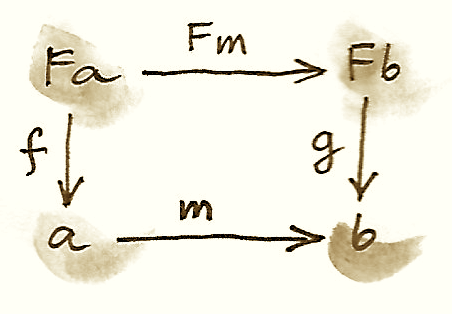
\includegraphics[width=2.09375in]{images/alg.png}

It's easy to convince yourself that this is indeed a category (hint:
identity morphisms from \emph{C} work just fine, and a composition of
homomorphisms is a homomorphism).

An initial object in the category of F-algebras, if it exists, is called
the \emph{initial algebra}. Let's call the carrier of this initial
algebra \texttt{i} and its evaluator
\texttt{j\ ::\ F\ i\ -\textgreater{}\ i}. It turns out that \texttt{j},
the evaluator of the initial algebra, is an isomorphism. This result is
known as Lambek's theorem. The proof relies on the definition of the
initial object, which requires that there be a unique homomorphism
\texttt{m} from it to any other F-algebra. Since \texttt{m} is a
homomorphism, the following diagram must commute:

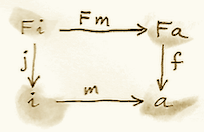
\includegraphics{images/alg2.png}

Now let's construct an algebra whose carrier is \texttt{F\ i}. The
evaluator of such an algebra must be a morphism from \texttt{F\ (F\ i)}
to \texttt{F\ i}. We can easily construct such an evaluator simply by
lifting \texttt{j}:

\begin{verbatim}
F j :: F (F i) -> F i
\end{verbatim}

Because \texttt{(i,\ j)} is the initial algebra, there must be a unique
homomorphism \texttt{m} from it to \texttt{(F\ i,\ F\ j)}. The following
diagram must commute:

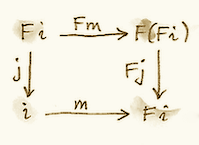
\includegraphics{images/alg3a.png}

But we also have this trivially commuting diagram (both paths are the
same!):

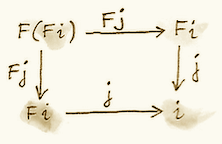
\includegraphics{images/alg3.png}

which can be interpreted as showing that \texttt{j} is a homomorphism of
algebras, mapping \texttt{(F\ i,\ F\ j)} to \texttt{(i,\ j)}. We can
glue these two diagrams together to get:

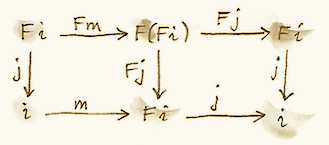
\includegraphics[width=3.12500in]{images/alg4.png}

This diagram may, in turn, be interpreted as showing that
\texttt{j\ ∘\ m} is a homomorphism of algebras. Only in this case the
two algebras are the same. Moreover, because \texttt{(i,\ j)} is
initial, there can only be one homomorphism from it to itself, and
that's the identity morphism \texttt{idi} --- which we know is a
homomorphism of algebras. Therefore \texttt{j\ ∘\ m\ =\ idi}. Using this
fact and the commuting property of the left diagram we can prove that
\texttt{m\ ∘\ j\ =\ idFi}. This shows that \texttt{m} is the inverse of
\texttt{j} and therefore \texttt{j} is an isomorphism between
\texttt{F\ i} and \texttt{i}:

\begin{verbatim}
F i ≅ i
\end{verbatim}

But that is just saying that \texttt{i} is a fixed point of \texttt{F}.
That's the formal proof behind the original hand-waving argument.

Back to Haskell: We recognize \texttt{i} as our \texttt{Fix\ f},
\texttt{j} as our constructor \texttt{Fix}, and its inverse as
\texttt{unFix}. The isomorphism in Lambek's theorem tells us that, in
order to get the initial algebra, we take the functor \texttt{f} and
replace its argument \texttt{a} with \texttt{Fix\ f}. We also see why
the fixed point does not depend on \texttt{a}.

\subsubsection{Natural Numbers}\label{natural-numbers}

Natural numbers can also be defined as an F-algebra. The starting point
is the pair of morphisms:

\begin{verbatim}
zero :: 1 -> N succ :: N -> N
\end{verbatim}

The first one picks the zero, and the second one maps all numbers to
their successors. As before, we can combine the two into one:

\begin{verbatim}
1 + N -> N
\end{verbatim}

The left hand side defines a functor which, in Haskell, can be written
like this:

\begin{verbatim}
data NatF a = ZeroF | SuccF a
\end{verbatim}

The fixed point of this functor (the initial algebra that it generates)
can be encoded in Haskell as:

\begin{verbatim}
data Nat = Zero | Succ Nat
\end{verbatim}

A natural number is either zero or a successor of another number. This
is known as the Peano representation for natural numbers.

\subsection{Catamorphisms}\label{catamorphisms}

Let's rewrite the initiality condition using Haskell notation. We call
the initial algebra \texttt{Fix\ f}. Its evaluator is the contructor
\texttt{Fix}. There is a unique morphism \texttt{m} from the initial
algebra to any other algebra over the same functor. Let's pick an
algebra whose carrier is \texttt{a} and the evaluator is \texttt{alg}.

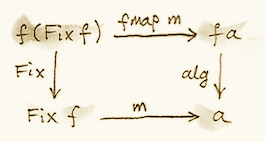
\includegraphics{images/alg5.png}\\
By the way, notice what \texttt{m} is: It's an evaluator for the fixed
point, an evaluator for the whole recursive expression tree. Let's find
a general way of implementing it.

Lambek's theorem tells us that the constructor \texttt{Fix} is an
isomorphism. We called its inverse \texttt{unFix}. We can therefore flip
one arrow in this diagram to get:

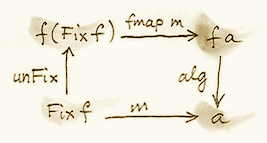
\includegraphics{images/alg6.png}

Let's write down the commutation condition for this diagram:

\begin{verbatim}
m = alg . fmap m . unFix
\end{verbatim}

We can interpret this equation as a recursive definition of \texttt{m}.
The recursion is bound to terminate for any finite tree created using
the functor \texttt{f}. We can see that by noticing that
\texttt{fmap\ m} operates underneath the top layer of the functor
\texttt{f}. In other words, it works on the children of the original
tree. The children are always one level shallower than the original
tree.

Here's what happens when we apply \texttt{m} to a tree constructed using
\texttt{Fix\ f}. The action of \texttt{unFix} peels off the constructor,
exposing the top level of the tree. We then apply \texttt{m} to all the
children of the top node. This produces results of type \texttt{a}.
Finally, we combine those results by applying the non-recursive
evaluator \texttt{alg}. The key point is that our evaluator \texttt{alg}
is a simple non-recursive function.

Since we can do this for any algebra \texttt{alg}, it makes sense to
define a higher order function that takes the algebra as a parameter and
gives us the function we called \texttt{m}. This higher order function
is called a catamorphism:

\begin{verbatim}
cata :: Functor f => (f a -> a) -> Fix f -> a cata alg = alg . fmap (cata alg) . unFix
\end{verbatim}

Let's see an example of that. Take the functor that defines natural
numbers:

\begin{verbatim}
data NatF a = ZeroF | SuccF a
\end{verbatim}

Let's pick \texttt{(Int,\ Int)} as the carrier type and define our
algebra as:

\begin{verbatim}
fib :: NatF (Int, Int) -> (Int, Int) fib ZeroF = (1, 1) fib (SuccF (m, n)) = (n, m + n)
\end{verbatim}

You can easily convince yourself that the catamorphism for this algebra,
\texttt{cata\ fib}, calculates Fibonacci numbers.

In general, an algebra for \texttt{NatF} defines a recurrence relation:
the value of the current element in terms of the previous element. A
catamorphism then evaluates the n-th element of that sequence.

\subsection{Folds}\label{folds}

A list of \texttt{e} is the initial algebra of the following functor:

\begin{verbatim}
data ListF e a = NilF | ConsF e a
\end{verbatim}

Indeed, replacing the variable \texttt{a} with the result of recursion,
which we'll call \texttt{List\ e}, we get:

\begin{verbatim}
data List e = Nil | Cons e (List e)
\end{verbatim}

An algebra for a list functor picks a particular carrier type and
defines a function that does pattern matching on the two constructors.
Its value for \texttt{NilF} tells us how to evaluate an empty list, and
its value for \texttt{ConsF} tells us how to combine the current element
with the previously accumulated value.

For instance, here's an algebra that can be used to calculate the length
of a list (the carrier type is \texttt{Int}):

\begin{verbatim}
lenAlg :: ListF e Int -> Int lenAlg (ConsF e n) = n + 1 lenAlg NilF = 0
\end{verbatim}

Indeed, the resulting catamorphism \texttt{cata\ lenAlg} calculates the
length of a list. Notice that the evaluator is a combination of (1) a
function that takes a list element and an accumulator and returns a new
accumulator, and (2) a starting value, here zero. The type of the value
and the type of the accumulator are given by the carrier type.

Compare this to the traditional Haskell definition:

\begin{verbatim}
length = foldr (\e n -> n + 1) 0
\end{verbatim}

The two arguments to \texttt{foldr} are exactly the two components of
the algebra.

Let's try another example:

\begin{verbatim}
sumAlg :: ListF Double Double -> Double sumAlg (ConsF e s) = e + s sumAlg NilF = 0.0
\end{verbatim}

Again, compare this with:

\begin{verbatim}
sum = foldr (\e s -> e + s) 0.0
\end{verbatim}

As you can see, \texttt{foldr} is just a convenient specialization of a
catamorphism to lists.

\subsection{Coalgebras}\label{coalgebras}

As usual, we have a dual construction of an F-coagebra, where the
direction of the morphism is reversed:

\begin{verbatim}
a -> F a
\end{verbatim}

Coalgebras for a given functor also form a category, with homomorphisms
preserving the coalgebraic structure. The terminal object
\texttt{(t,\ u)} in that category is called the terminal (or final)
coalgebra. For every other algebra \texttt{(a,\ f)} there is a unique
homomorphism \texttt{m} that makes the following diagram commute:

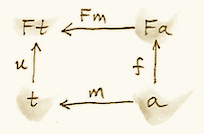
\includegraphics{images/alg7.png}

A terminal colagebra is a fixed point of the functor, in the sense that
the morphism \texttt{u\ ::\ t\ -\textgreater{}\ F\ t} is an isomorphism
(Lambek's theorem for coalgebras):

\begin{verbatim}
F t ≅ t
\end{verbatim}

A terminal coalgebra is usually interpreted in programming as a recipe
for generating (possibly infinite) data structures or transition
systems.

Just like a catamorphism can be used to evaluate an initial algebra, an
anamorphism can be used to coevaluate a terminal coalgebra:

\begin{verbatim}
ana :: Functor f => (a -> f a) -> a -> Fix f ana coalg = Fix . fmap (ana coalg) . coalg
\end{verbatim}

A canonical example of a coalgebra is based on a functor whose fixed
point is an infinite stream of elements of type \texttt{e}. This is the
functor:

\begin{verbatim}
data StreamF e a = StreamF e a deriving Functor
\end{verbatim}

and this is its fixed point:

\begin{verbatim}
data Stream e = Stream e (Stream e)
\end{verbatim}

A coalgebra for \texttt{StreamF\ e} is a function that takes the seed of
type \texttt{a} and produces a pair (\texttt{StreamF} is a fancy name
for a pair) consisting of an element and the next seed.

You can easily generate simple examples of coalgebras that produce
infinite sequences, like the list of squares, or reciprocals.

A more interesting example is a coalgebra that produces a list of
primes. The trick is to use an infinite list as a carrier. Our starting
seed will be the list \texttt{{[}2..{]}}. The next seed will be the tail
of this list with all multiples of 2 removed. It's a list of odd numbers
starting with 3. In the next step, we'll take the tail of this list and
remove all multiples of 3, and so on. You might recognize the makings of
the sieve of Eratosthenes. This coalgebra is implemented by the
following function:

\begin{verbatim}
era :: [Int] -> StreamF Int [Int] era (p : ns) = StreamF p (filter (notdiv p) ns) where notdiv p n = n `mod` p /= 0
\end{verbatim}

The anamorphism for this coalgebra generates the list of primes:

\begin{verbatim}
primes = ana era [2..]
\end{verbatim}

A stream is an infinite list, so it should be possible to convert it to
a Haskell list. To do that, we can use the same functor \texttt{StreamF}
to form an algebra, and we can run a catamorphism over it. For instance,
this is a catamorphism that converts a stream to a list:

\begin{verbatim}
toListC :: Fix (StreamF e) -> [e] toListC = cata al where al :: StreamF e [e] -> [e] al (StreamF e a) = e : a
\end{verbatim}

Here, the same fixed point is simultaneously an initial algebra and a
terminal coalgebra for the same endofunctor. It's not always like this,
in an arbitrary category. In general, an endofunctor may have many (or
no) fixed points. The initial algebra is the so called least fixed
point, and the terminal coalgebra is the greatest fixed point. In
Haskell, though, both are defined by the same formula, and they
coincide.

The anamorphism for lists is called unfold. To create finite lists, the
functor is modified to produce a \texttt{Maybe} pair:

\begin{verbatim}
unfoldr :: (b -> Maybe (a, b)) -> b -> [a]
\end{verbatim}

The value of \texttt{Nothing} will terminate the generation of the list.

An interesting case of a coalgebra is related to lenses. A lens can be
represented as a pair of a getter and a setter:

\begin{verbatim}
set :: a -> s -> a get :: a -> s
\end{verbatim}

Here, \texttt{a} is usually some product data type with a field of type
\texttt{s}. The getter retrieves the value of that field and the setter
replaces this field with a new value. These two functions can be
combined into one:

\begin{verbatim}
a -> (s, s -> a)
\end{verbatim}

We can rewrite this function further as:

\begin{verbatim}
a -> Store s a
\end{verbatim}

where we have defined a functor:

\begin{verbatim}
data Store s a = Store (s -> a) s
\end{verbatim}

Notice that this is not a simple algebraic functor constructed from sums
of products. It involves an exponential \texttt{as}.

A lens is a coalgebra for this functor with the carrier type \texttt{a}.
We've seen before that \texttt{Store\ s} is also a comonad. It turns out
that a well-behaved lens corresponds to a coalgebra that is compatible
with the comonad structure. We'll talk about this in the next section.

\subsection{Challenges}\label{challenges}

\begin{enumerate}
\tightlist
\item
  Implement the evaluation function for a ring of polynomials of one
  variable. You can represent a polynomial as a list of coefficients in
  front of powers of \texttt{x}. For instance, \texttt{4x2-1} would be
  represented as (starting with the zero'th power)
  \texttt{{[}-1,\ 0,\ 4{]}}.
\item
  Generalize the previous construction to polynomials of many
  independent variables, like \texttt{x2y-3y3z}.
\item
  Implement the algebra for the ring of 2×2 matrices.
\item
  Define a coalgebra whose anamorphism produces a list of squares of
  natural numbers.
\item
  Use \texttt{unfoldr} to generate a list of the first \texttt{n}
  primes.
\end{enumerate}

Next:
\href{https://bartoszmilewski.com/2017/03/14/algebras-for-monads/}{Algebras
for Monads}.
